\section{CrashSimulator Approach Details}
    %%% This figure is definitely wrong. Will recreate %%%
    \begin{figure*}[t]
        \center{}
        \fbox{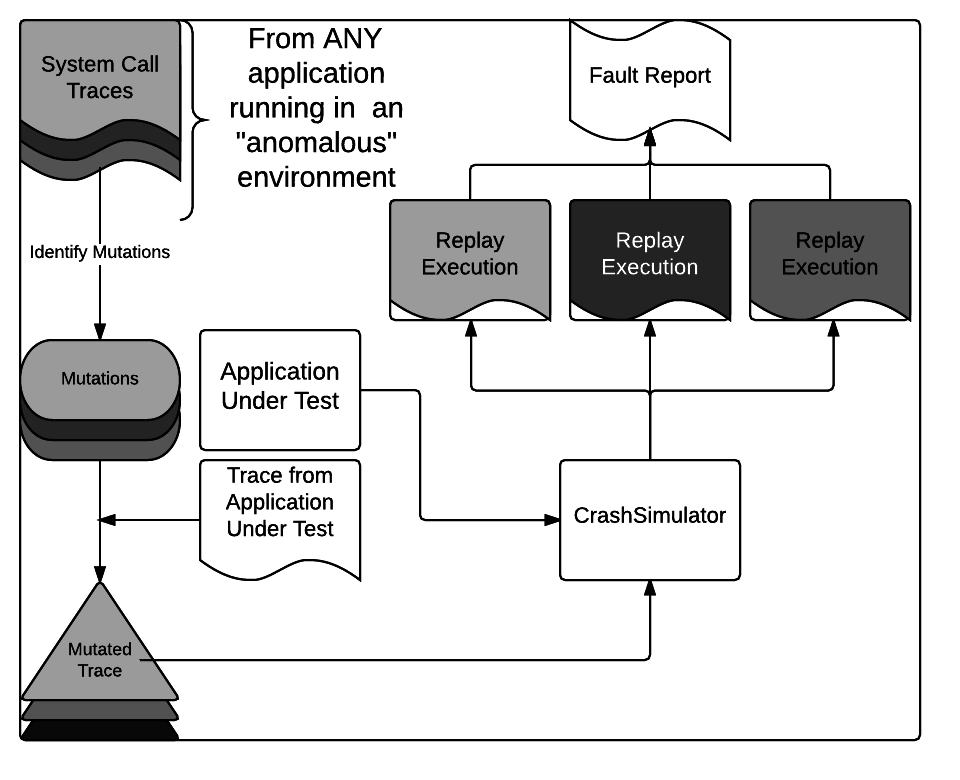
\includegraphics[scale=.5]{Architecture}}
        \caption{\emph{We need a new figure.}}

    \end{figure*}

    \subsection{Architecture}
        
    At a high level CrashSimulator is organized into three primary modules. The first module is responsible for
    monitoring a given execution, determining when to inject anomalous behavior, determining whether or not the
    application responded correctly to the injected behavior. The second module is responsible for managing the
    execution of the application under test such that it precisely follows a previously recorded system call trace -- a
    process we refer to as ``replaying'' a system call trace. The third module orchestrates the process of running
    multiple different anomalies against the application under test, much like a unit test suite.
        
    The first step in CrashSimulator's work flow is to identify anomalous behavior in an arbitrary application. For the
    purposes of this work, this step is accomplished through manual bug hunting and through examination of diagnostic
    output from NetCheck and CheckAPI. CrashSimulator's user examines the system call behavior that resulted in this bad
    behavior and constructs a model defines what triggers the anomalous behavior and the subsequent ``bad'' system call
    behavior (\emph{Do we need to say something about future work doing this step automatically here?}.
    CrashSimulator's first module operates by using this model to analyzed the system call behavior of the application
    under test(e.g. order, parameters, side effects, return values).
        
    CrashSimulator's second module makes use of the Ptrace facilities built into modern versions of the Linux
    kernel. The aforementioned ``replay'' of a system call trace is achieved by intercepting every system call the
    application makes, preventing the actual system call from being carried out by the kernel (i.e. no-oping out the
    real system call, that is replacing it with a call to getpid()), identifying the matching system call from the
    previously recorded trace, and replicating the return value and side effects such that the application believes that
    the system call it made actually took place. We have found that faithfully emulating the post conditions of the
    system calls an application makes results in deterministic replay of a previous execution in most cases.

    Replay is important because it allows CrashSimulator to execute an application free from dependencies on things like
    file system contents, network configuration, or communication with other applications....... \emph{need more here
      -Preston}

    All three primary CrashSimulator modules are packaged together and interact with each other at the appropriate times
    without user intervention. At this point, CrashSimulator itself is available as a virtual machine appliance
    compatible with the \emph{Virtual Box} virtual machine hosting software. The reasons for distributing CrashSimulator
    in this manner are threefold. First, this distribution method ensures that all of CrashSimulator's dependences are
    installed and configured appropriately. Second, this method provides an environment for taking system call traces
    that is known to be complete tool-wise and compatible with CrashSimulator. Finally, and most importantly, this
    method provides an environment that is known to be compatible with the details of CrashSimulator's system call
    replay techniques.

    CrashSimulator's source code is available and, while other environments may be untested, it should function
    correctly on any platforms that meet the criteria described above.

    \subsection{Anomaly Identification}
    
    \emph{This is an old paragraph but I'm leaving it in because I think the general idea it conveys is
      good. -Preston}The first step in CrashSimulator's operation is the analysis of the set of input system call traces
    recorded from other applications running in the intended deployment environment. These traces can be taken from any
    application that as environmental requirements that are reasonably similar to the application under test. For
    example, a web server could likely be effectively tested by CrashSimulator when CrashSimulator is given system call
    traces from other applications that make heavy use of the network. Testing a web browser with traces from an
    application that has no network usage at all would result in less effective testing.
    
    A variety of tools capable of identifying anomalies usable by CrashSimulator already exist. This work relies on
    NetCheck and CheckAPI for this purpose. NetCheck readily able to identify a wide variety of anomalous behaviors
    related to network communication between one or more hosts. During normal operation, NetCheck analyzes a group of
    input system call traces and attempts to produce a diagnosis for network related faults. These faults can be
    analyzed by CrashSimulator's user so that models that encode them can be constructed. CheckAPI peforms a similar
    function by comparing ``behavior of an API implementation to a reference model.''
    
    Additionally, models were constructed that encoded issues identified through manual bug hunting. Specifically,
    we constructed models that identified bad behavior around moving files from one filesystem to another. Using these
    models, CrashSimulator was identify when applications (nodejs etc.) performed this operation incorrectly.

    This process of identifying anomalies does not need to be performed for each run of the test suite.  CrashSimulator
    maintains a corpus of anomalies it has extracted from sample traces. These anomalies can be used to produce mutated
    traces for any future application that it tests. This allows a developer to build up a set of anomalies that were
    identified from each of their target environments. The developer can then test an application against this set of
    anomalies and get an idea of how their application will behave should it encounter the anomalies a deployment
    environment.

    \subsection{System Call Traces and Replay}

        \subsubsection{Why System Call Traces?}

        In order to inject anomalies and monitor program behavior as described above, CrashSimulator needs to have detailed
        interactions with the application under test at some level.  The option of carrying out these interactions at the
        system call level was chosen because for several reasons:

        \paragraph{Tooling}

        Operating at the system call level allows this work to take advantage of two key pieces of tooling that already
        exist in mature form on Linux.  The first is ptrace. Ptrace is an process manipulation interface provided by the
        Linux kernel whose primary use case is debugger development.  This work leverages ptrace in order to start and stop
        execution of a process as well as read and write the contents of the processes registers and memory.  Using these
        operations allows CrashSimulator to pause execution before and after each system call an application makes in order
        to manage execution and inject anomalies where appropriate.

        This CrashSimulator also relies on system call traces recorded using strace.  The strace system call trace format is
        extensive and captures the parameters, return values, and side effects of each system call an application makes.
        Such a record provides CrashSimulator with all the information needed to direct execution of the application in such
        a way that the contents of the system call trace are faithfully replayed.  It is in this way that system call traces
        act as an interface over an applications execution that used to inject anomalous behavior.

        \paragraph{Removal of language dependence}

        Operating at the system call level means that CrashSimulator is not dependant on a particular programming
        language or runtime.  This means that CrashSimulator does not require any complext language parsing and analysis
        while still posessing many of the benefits of systems that perform such work.  Tools that perform language
        parsing do so in order to craft inputs that specifically exercise target execution paths in an application.
        This work is concerned with issues that arise at the ``interfaces'' between an application and its environment.
        Manipulating system calls allows us to skip the process of generating these inputs in favor of directly
        effecting the behavior we are interested in.

        \paragraph{Identify Issues that Result from an Application's Environment}

        Most current testing strategies are very application-centric.  For example, a black box fuzzer is able to
        identify faults that arise when an application begins processing data it has received from a network
        connection. CrashSimulator, on the other hand, is able to identify issues that arisese from the network connection
        itself.

    \subsubsection{Why Replay Executions?}

    \emph{I need to quit saying ``For Example'' so much -Preston}

    \paragraph{Removal of Dependencies}

    Replaying an execution allows CrashSimulator, in many cases, to completely simulate some aspect of an applications
    environment using the data recorded in a system call trace from a previous application.  For example, if an
    application depends on a file being present in a filesystem, CrashSimulator can intercept calls to read()
    from / write() to this file alleviating the need this file to actually be present during replay executions.

    \paragraph{Control Execution}

    Because it is simulating aspects the application under test's environment, CrashSimulator is able to manipulate the
    data the application receives from these aspects in order to control execution.  This is the key feature that allows
    CrashSimulator to inject anomalous situations into an execution.  For example, by simulating the communications
    between the application under test and another host on a network, CrashSimulator can fragment, modify, or even drop
    data ``incoming'' from the simulated remote host in order to determine whether or not the application appropriately
    handles the situation. 
    
    \paragraph{Making Determinations About Program Behavior}

    From a system call perspective, replaying an application implies that the application makes the same system calls
    with the same parameters in the same order as is present in the system call trace being used to drive the replay.
    If CrashSimulator injects behavior that \emph{should} necesistate some deviant behavior but the application
    continues along the the same execution path as is recorded in the system call trace then the application has not
    properly handled the injected bejavior.  For example, if CrashSimulator modifies the data structure ``returned'' by
    a call to stat64() such that the target file appears to be a symlink rather than a regular file and the application
    being replayed does not alter its behavior to deal with this fact, the application has not correctly handled the
    injected behavior -- a failing result.  Alternatively, if the application deivates from the behavior described in
    the system call trace driving the replay it is likely that the application is taking some action to handle the
    injected condition -- an indiciation of possibly correct behavior.